\documentclass[10pt]{article}
\usepackage[margin=0.65in]{geometry}
\usepackage{graphicx}
\usepackage{parskip}
\usepackage{microtype}

\title{\vspace{-2em}BMI/CS 771 Assignment 1: Image Processing Using Python}
\author{}
\date{}

\begin{document}
\maketitle
\vspace{-2.5em}

\section*{Overview}
The goal of this assignment was to implement three image transformations and
use them in a data augmentation pipeline for a small image-classification
problem. I completed the missing parts of \texttt{student\_code.py}, generated
the requested augmented image results, and ran the provided cat-versus-dog
training notebook from beginning to end.

\section*{Implementation}
\textbf{Scaling.} When the requested size is one integer, my implementation
sets the shorter side of the image to that value and computes the other side
from the original aspect ratio. When an exact width and height are given, the
image is resized directly to those dimensions. The provided interpolation
choice is passed to OpenCV in both cases.

\textbf{Color adjustment.} I sample an independent adjustment for each color
channel and multiply that channel by a value in
$[1-r,\,1+r]$. The calculation is performed in floating point to avoid
unsigned-integer overflow. I then clip the result to the valid pixel range
$[0,255]$ and convert it back to the input image's data type.

\textbf{Rotation.} I sample an angle from the requested range and construct an
OpenCV affine rotation around the image center. The rotation canvas is expanded
so that the image is not clipped. Finally, I calculate and extract the largest
centered axis-aligned rectangle containing no empty border pixels introduced by
the rotation.

\section*{Pipeline and Results}
For the visualization pipeline, the notebook combines scaling, horizontal
flipping, color adjustment, rotation, and random cropping. The four saved
output strips show ten augmented versions of each source image. The examples
retain the original subject while introducing useful variation in orientation,
crop, and color:

\begin{center}
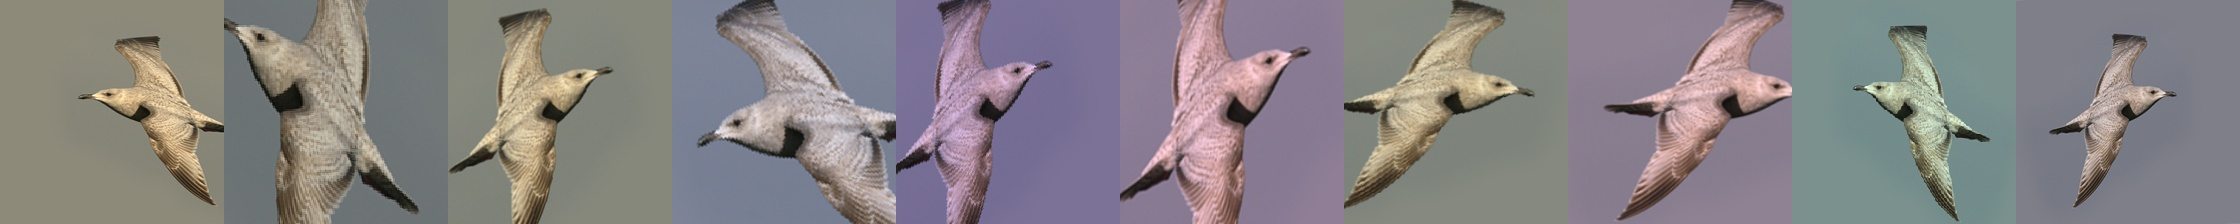
\includegraphics[width=0.96\textwidth]{../results/outputs_1.jpg}\\[0.35em]
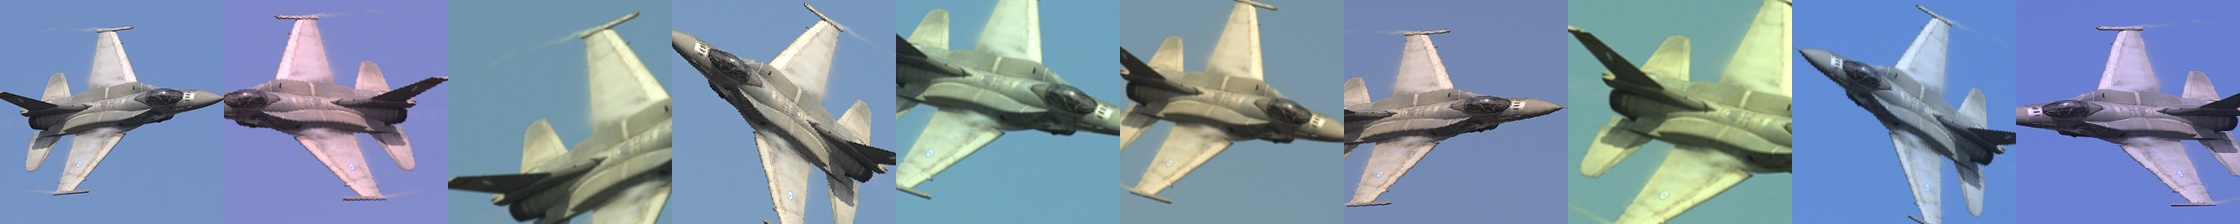
\includegraphics[width=0.96\textwidth]{../results/outputs_3.jpg}
\end{center}

For model training, images are scaled, randomly flipped, randomly cropped to
$64\times64$, and converted to tensors. Validation images use a deterministic
center crop instead. The supplied neural network was trained for six epochs on
the CPU using cross-entropy loss and AdamW. The recorded validation accuracy
was \textbf{73\%}. The training loss generally decreased from about 0.69 near
the start to roughly 0.47--0.50 near the end, although individual minibatches
varied. Overall, the output images show that the completed transforms create
substantial visual diversity without changing class identity. Because the
pipeline uses random sampling, the exact images and accuracy can vary slightly
between runs.

\end{document}
